\chapter{Executing "Word Count" using the scala terminal}
\par In this section we will 
%Intro\footnotemark\\
\begin{spacing}{1.2}
%note en bas de page
\section{Connecting Spark to a Hadoop Distribution}

\par Spark can use the Hadoop client libraries for HDFS and YARN. We must modify SPARK_DIST_CLASSPATH to include the jar files relating to these packages.
\\
\begin{figure}[!htb] 
\begin{center} 
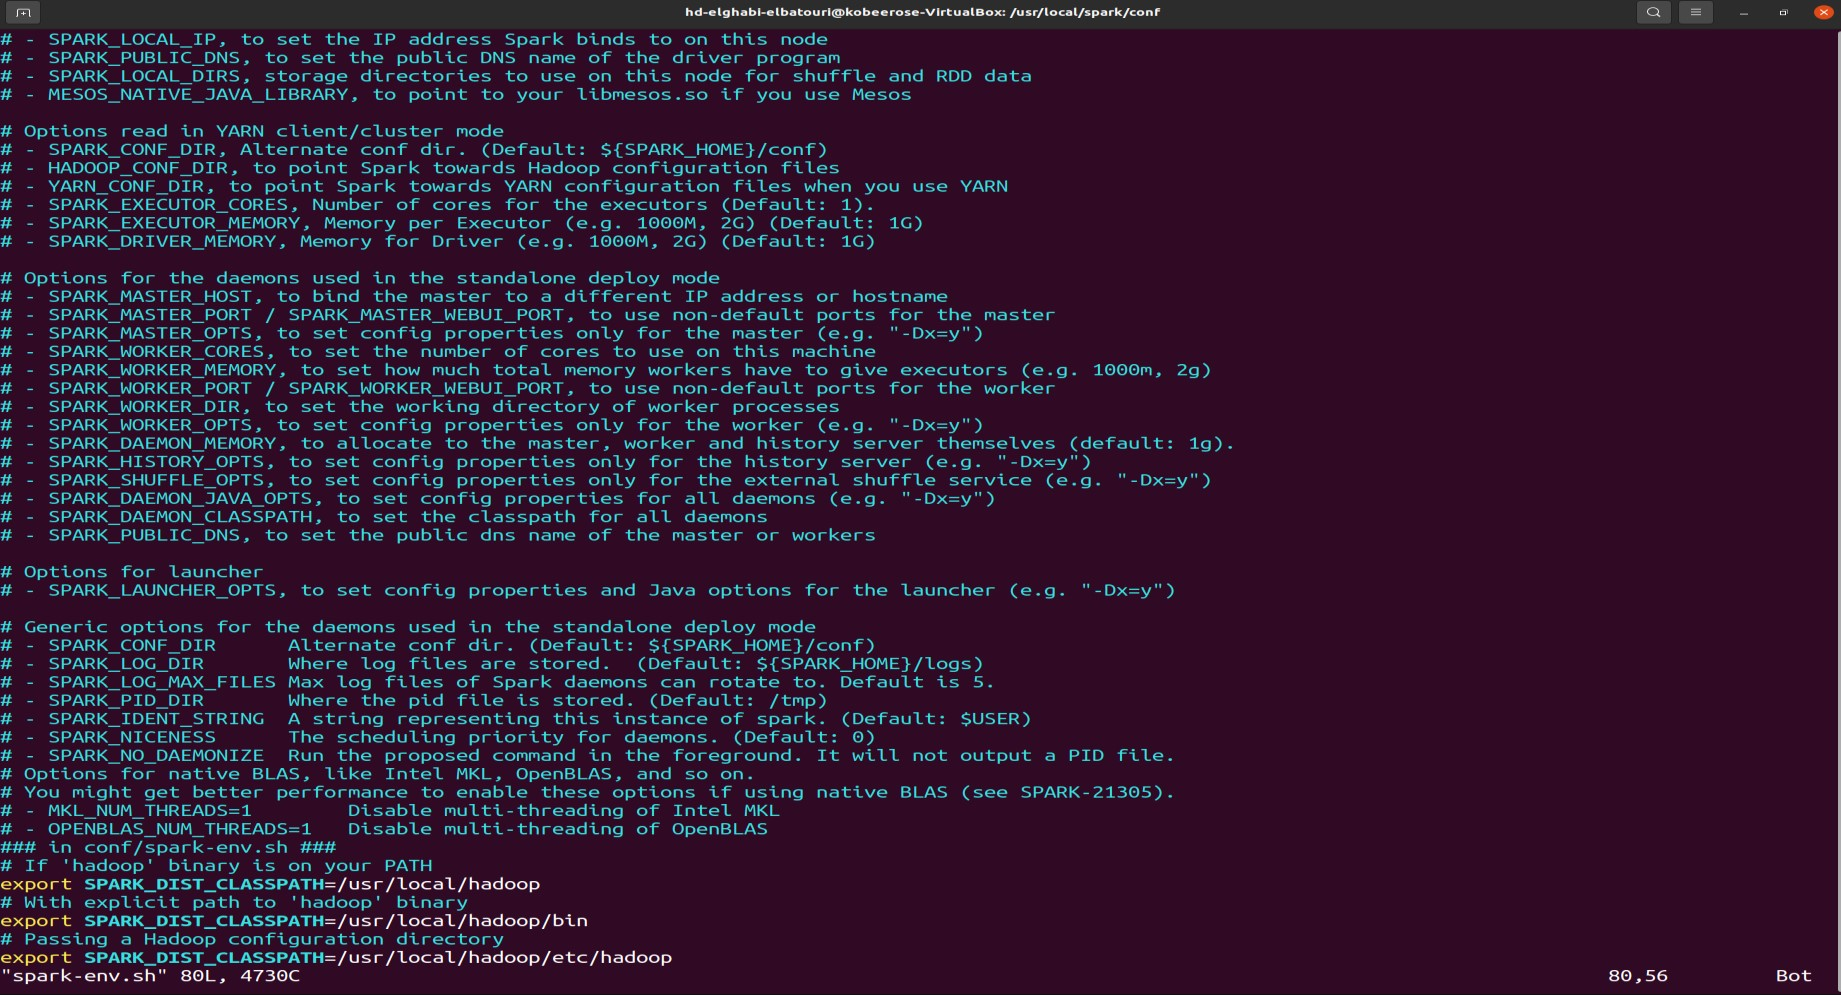
\includegraphics[width=1\linewidth]{Big_Data/Spark/Connecting Spark to Hadoop/spark-env config} 
\end{center} 
\caption{spark-env config} 
\end{figure} 
\FloatBarrier



\par Once the hadoop node is properly configured and spark well connected to hadoop. We can deposit data
in HDFS and use them by spark.
\\
\begin{figure}[!htb] 
\begin{center} 
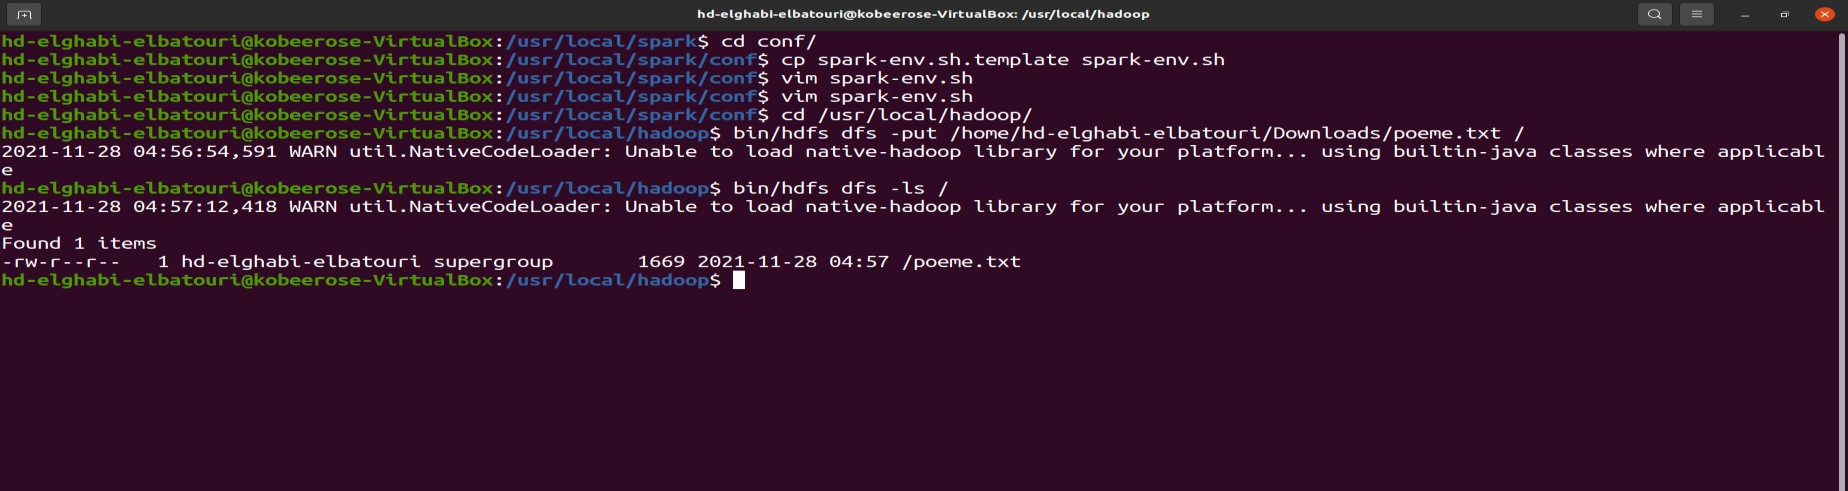
\includegraphics[width=1\linewidth]{Big_Data/Spark/Executing WCount using scala/Putting poeme.txt in hdfs} 
\end{center} 
\caption{Putting poeme.txt in hdfs} 
\end{figure} 
\FloatBarrier

\section{Executing of the "Word Count" code}

\par let's execute the "Word Count" processing using the spark-shell terminal
\\
\begin{figure}[!htb] 
\begin{center} 
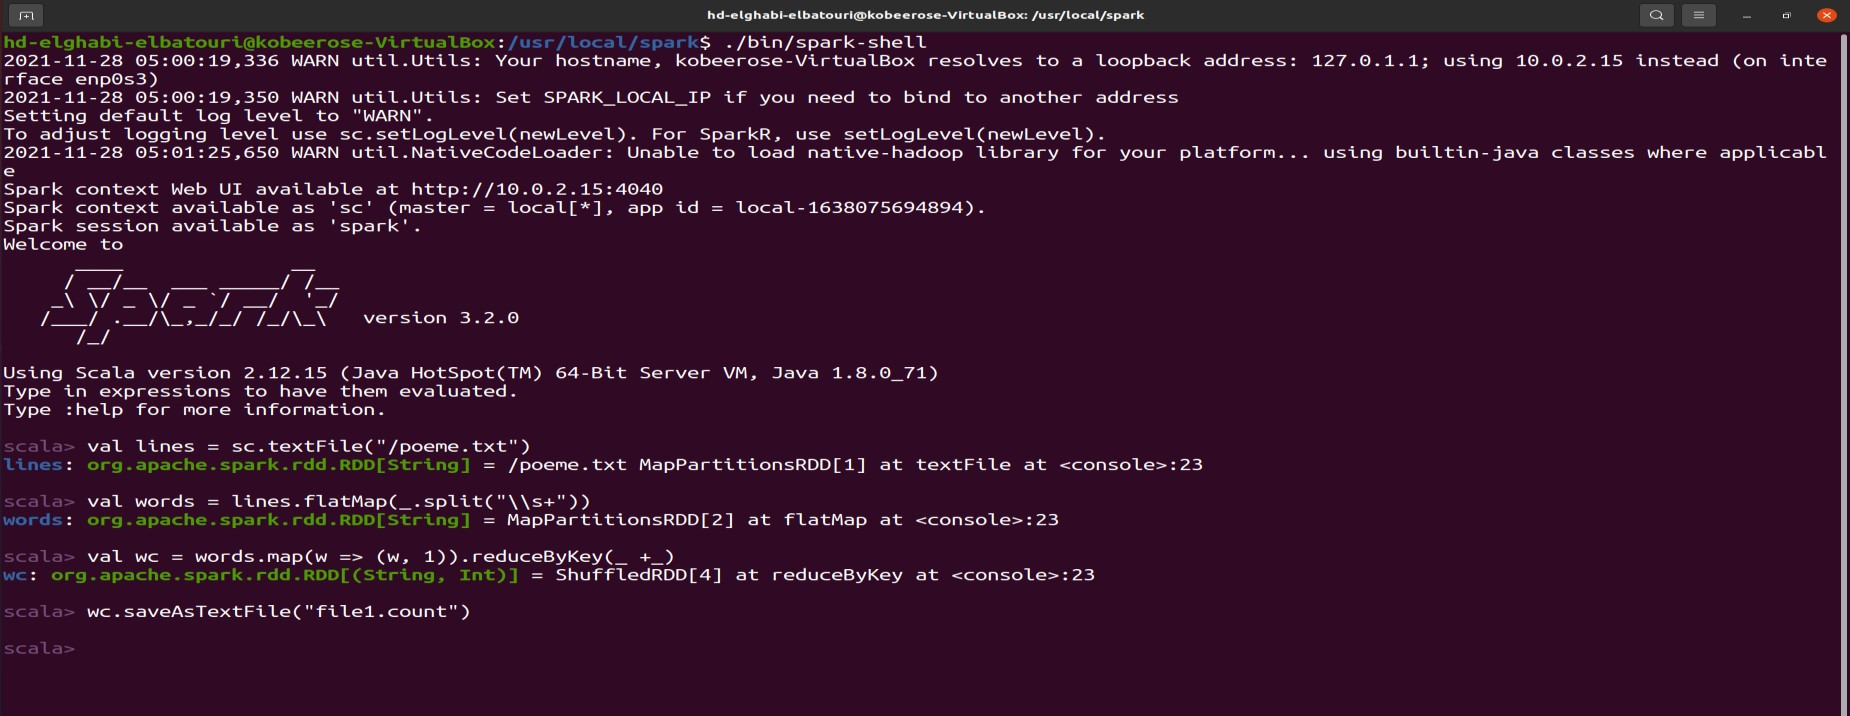
\includegraphics[width=1\linewidth]{Big_Data/Spark/Executing WCount using scala/Executing WCout} 
\end{center} 
\caption{Executing WCout} 
\end{figure} 
\FloatBarrier



\par The results of word count execution.
\\
\begin{figure}[!htb] 
\begin{center} 
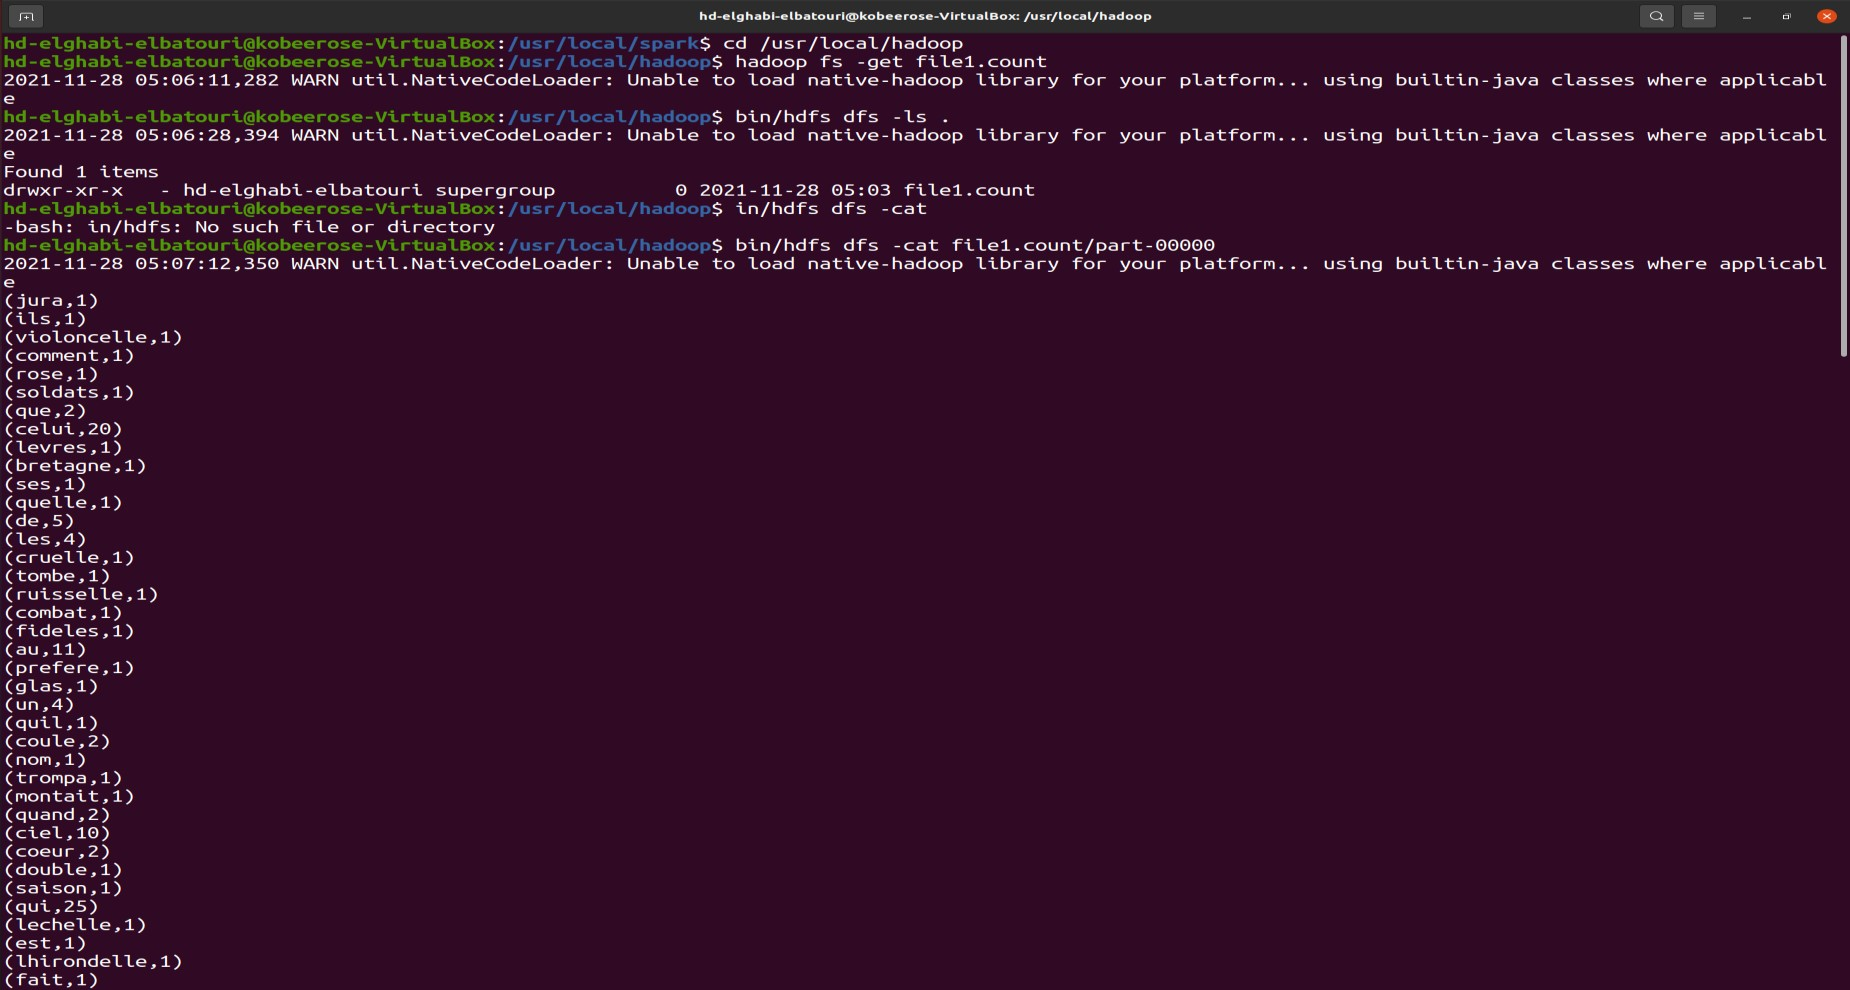
\includegraphics[width=1\linewidth]{Big_Data/Spark/Executing WCount using scala/WCount Results} 
\end{center} 
\caption{WCount Results} 
\end{figure} 
\FloatBarrier



\par Ley's perform the "Word Count" processing using the Pyspark terminal,
\\
\begin{figure}[!htb] 
\begin{center} 
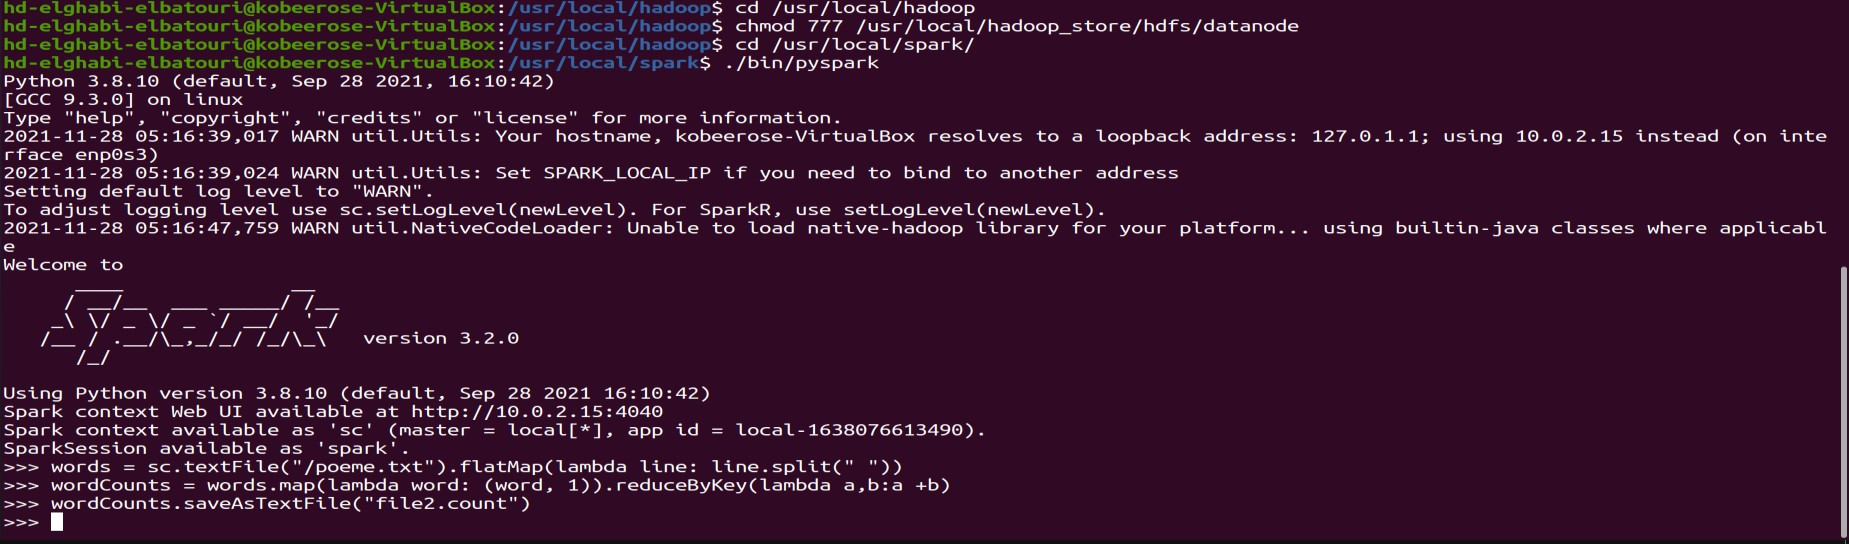
\includegraphics[width=1\linewidth]{Big_Data/Spark/Executing WCount using scala/WCout using pyspark} 
\end{center} 
\caption{WCout using pyspark} 
\end{figure} 
\FloatBarrier



\par Here is the results.
\\
\begin{figure}[!htb] 
\begin{center} 
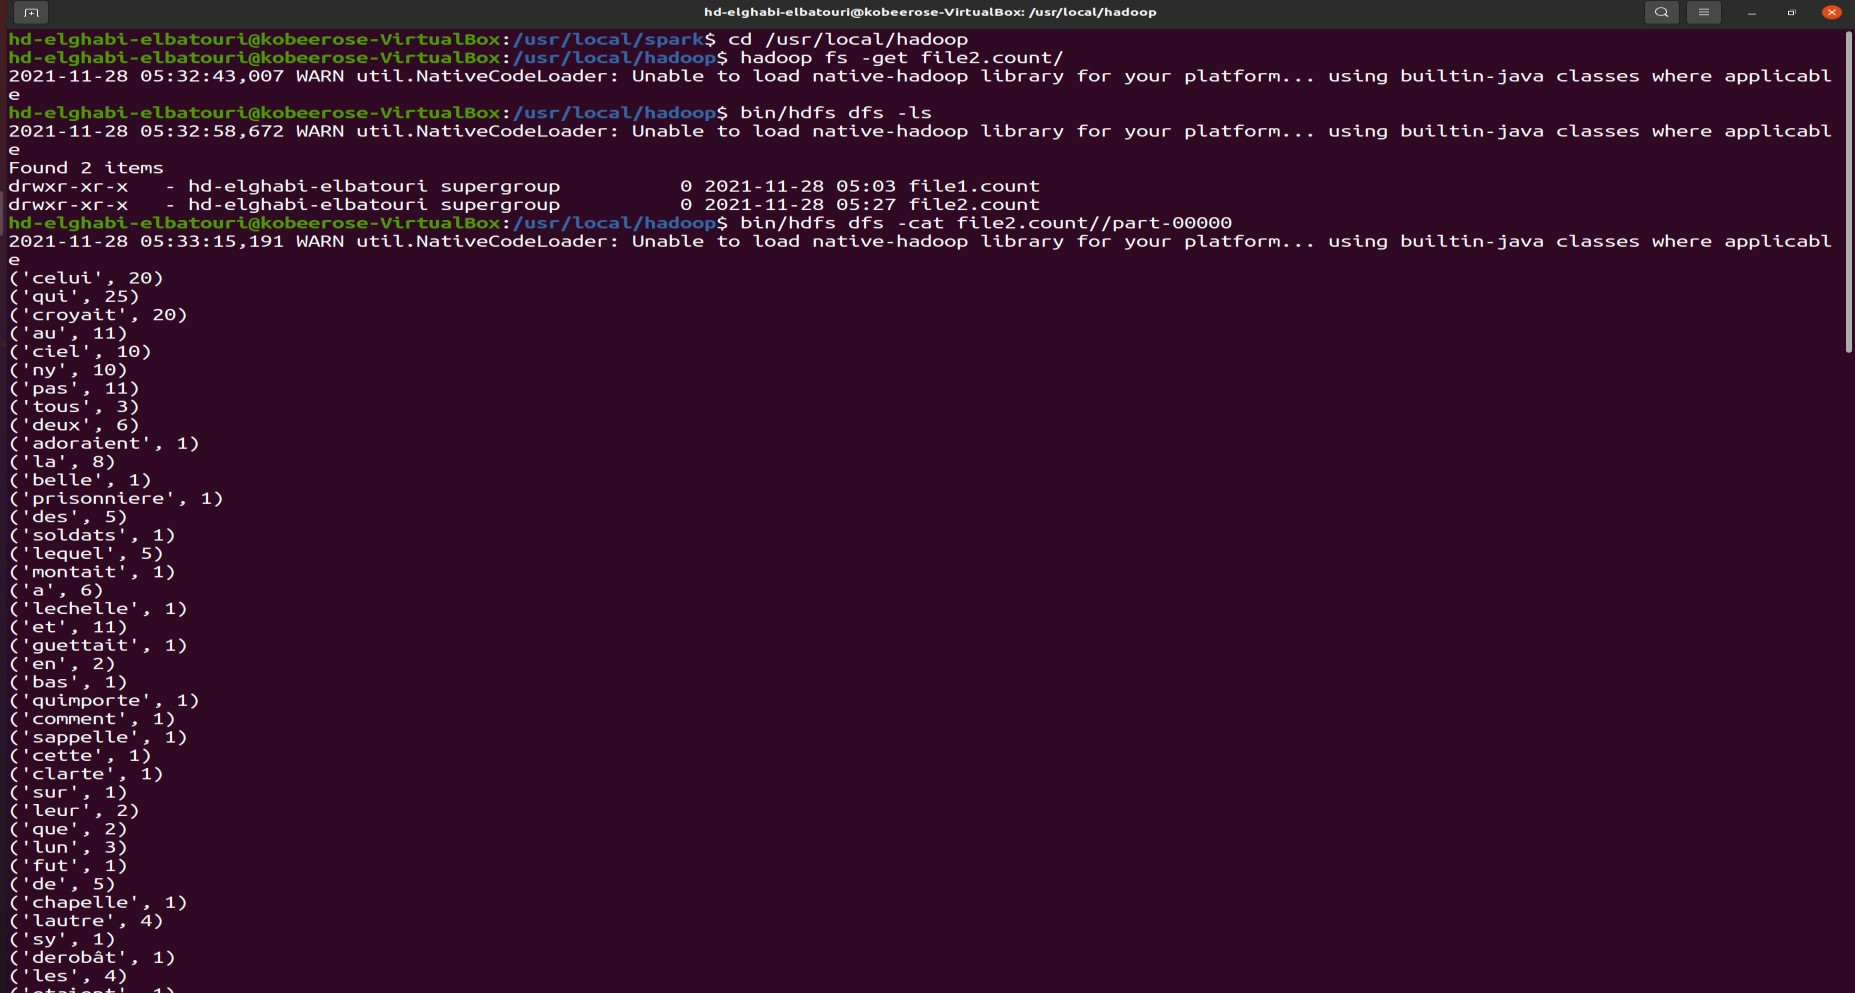
\includegraphics[width=1\linewidth]{Big_Data/Spark/Executing WCount using scala/WCout using pyspark Results} 
\end{center} 
\caption{WCout using pyspark Results} 
\end{figure} 
\FloatBarrier

\section{Execution of the "Word Count" using a python script}

\par We first Create a "word count.py" file in which we will have our python script to run.
\\
\begin{figure}[!htb] 
\begin{center} 
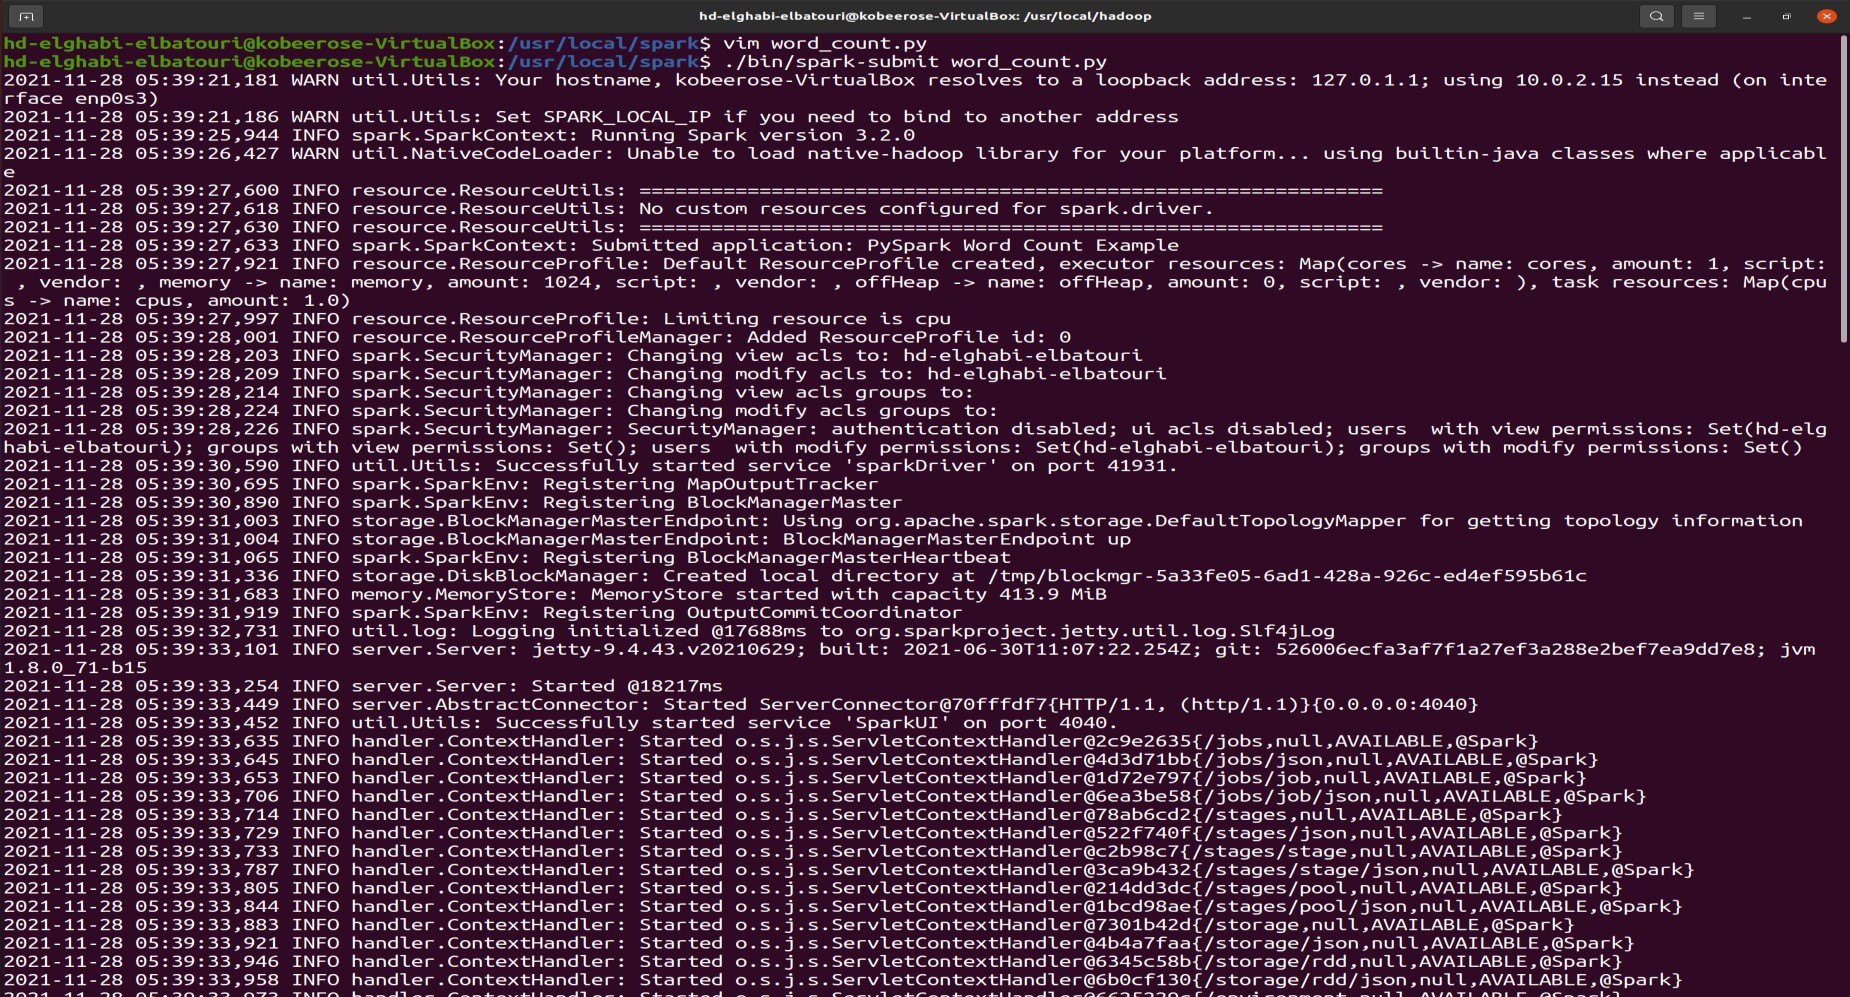
\includegraphics[width=1\linewidth]{Big_Data/Spark/Executing Word_Count using python/running a python script} 
\end{center} 
\caption{running a python script} 
\end{figure} 
\FloatBarrier


\par let's see the result of the script.

\\
\begin{figure}[!htb] 
\begin{center} 
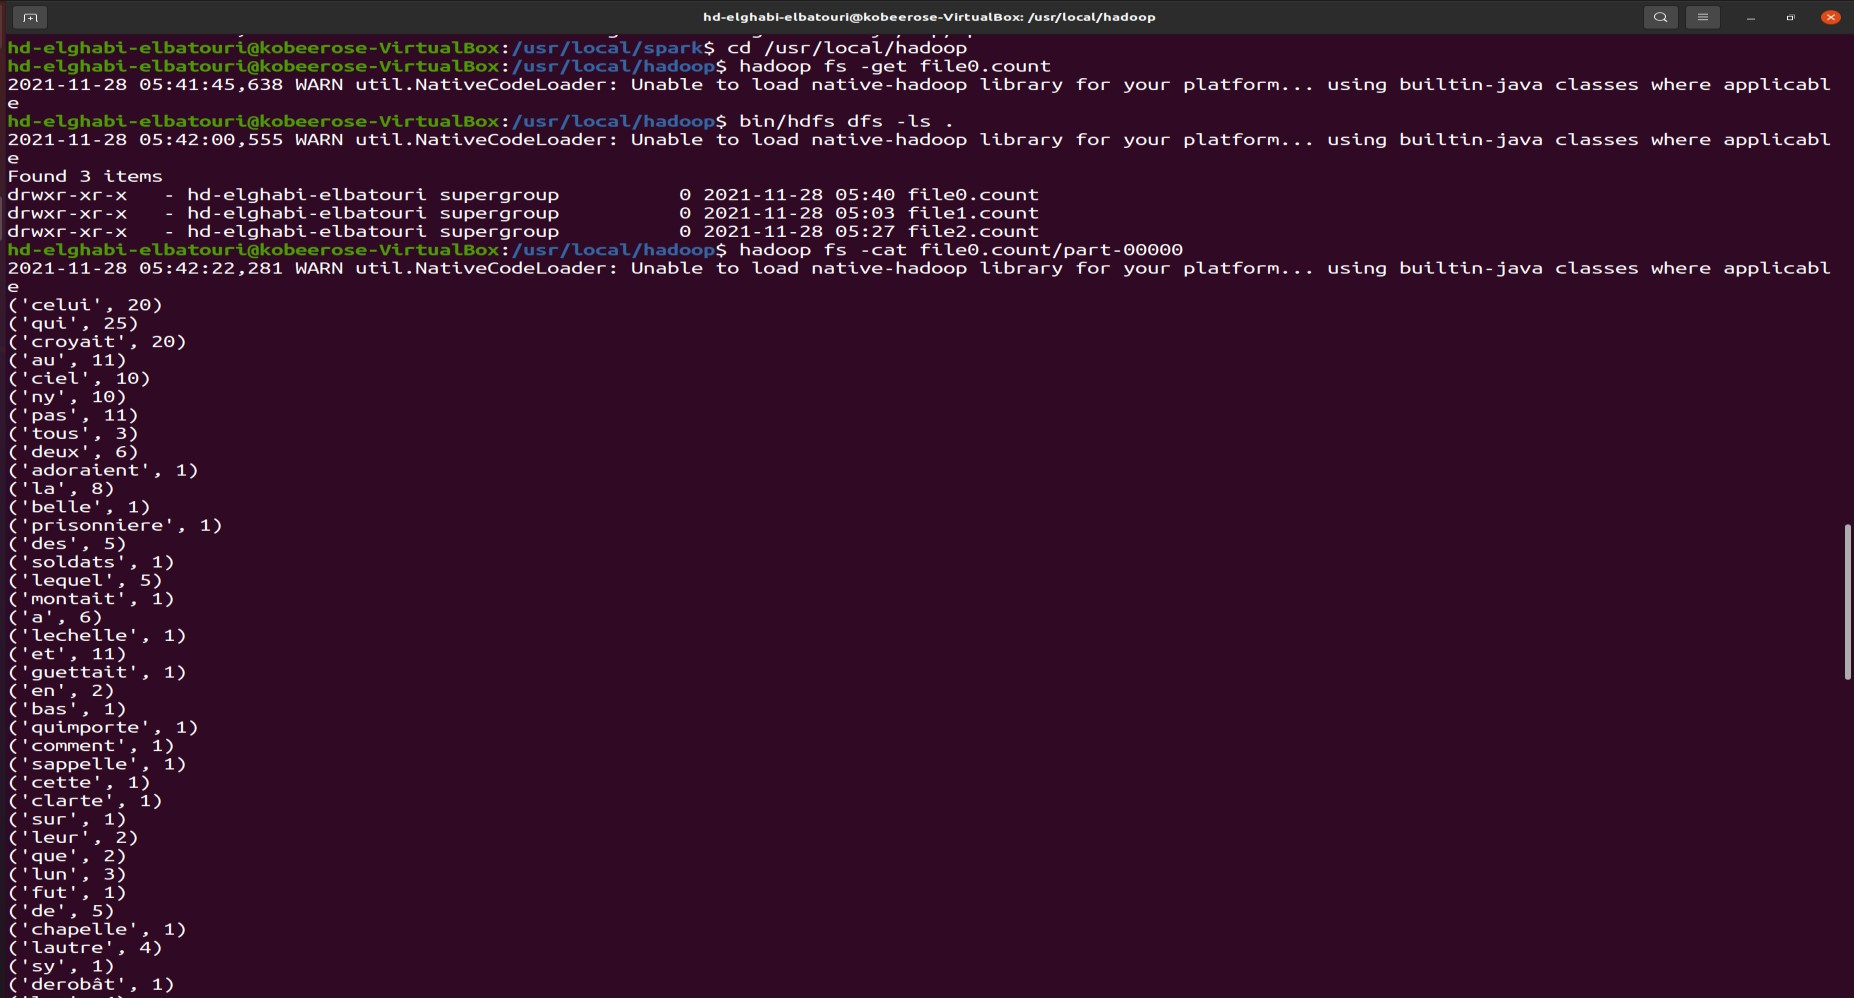
\includegraphics[width=1\linewidth]{Big_Data/Spark/Executing Word_Count using python/results of python script} 
\end{center} 
\caption{results of python script} 
\end{figure} 
\FloatBarrier



\end{spacing}